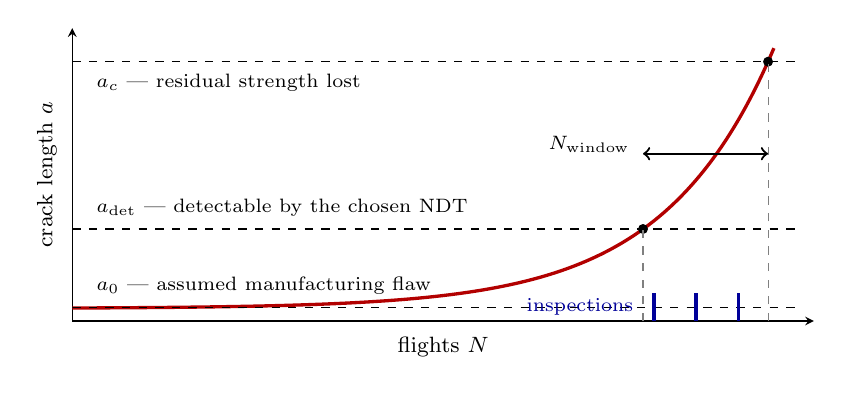
\begin{tikzpicture}
\begin{axis}[width=11.0cm,height=5.3cm,xlabel={flights $N$},ylabel={crack length $a$},
 xmin=0,xmax=1.02,ymin=0,ymax=1.05,xtick=\empty,ytick=\empty,axis lines=left,
 label style={font=\footnotesize}]
\addplot[very thick,red!70!black,domain=0:0.965,samples=240]{0.045+0.0016*exp(6.6*x)};
\draw[dashed] (axis cs:0,0.93) -- (axis cs:1.0,0.93);
\node[font=\scriptsize,anchor=north west] at (axis cs:0.02,0.92) {$a_c$ --- residual strength lost};
\draw[dashed] (axis cs:0,0.33) -- (axis cs:1.0,0.33);
\node[font=\scriptsize,anchor=south west] at (axis cs:0.02,0.34) {$a_{\mathrm{det}}$ --- detectable by the chosen NDT};
\draw[dashed] (axis cs:0,0.047) -- (axis cs:1.0,0.047);
\node[font=\scriptsize,anchor=south west] at (axis cs:0.02,0.06) {$a_0$ --- assumed manufacturing flaw};
% detectable / critical crossings
\fill (axis cs:0.785,0.33) circle (1.8pt);
\fill (axis cs:0.957,0.93) circle (1.8pt);
\draw[gray,dashed] (axis cs:0.785,0) -- (axis cs:0.785,0.33);
\draw[gray,dashed] (axis cs:0.957,0) -- (axis cs:0.957,0.93);
% window
\draw[<->,thick] (axis cs:0.785,0.60) -- (axis cs:0.957,0.60);
\node[font=\scriptsize,anchor=south east,align=right] at (axis cs:0.78,0.57) {$N_{\mathrm{window}}$};
% inspections
\draw[blue!60!black,very thick] (axis cs:0.800,0.0) -- (axis cs:0.800,0.10);
\draw[blue!60!black,very thick] (axis cs:0.858,0.0) -- (axis cs:0.858,0.10);
\draw[blue!60!black,very thick] (axis cs:0.916,0.0) -- (axis cs:0.916,0.10);
\node[font=\scriptsize,blue!60!black,anchor=east] at (axis cs:0.785,0.05) {inspections};
\end{axis}
\end{tikzpicture}